\documentclass[12pt]{article}

\usepackage[english]{babel}
\usepackage[T1]{fontenc}
\usepackage[utf8x]{inputenc}
\usepackage{amsmath,commath}
\usepackage{amssymb}
\usepackage{caption}
\usepackage{graphicx,subfig}
\usepackage[colorinlistoftodos]{todonotes}
\usepackage{tikz}
\usepackage[a4paper, left = 1in, right=1in, top=1in, bottom=1in]{geometry}
\usepackage{amssymb}
\usepackage{enumerate}
\usepackage{enumitem}
\usepackage{float}
\usepackage[bottom]{footmisc}
\usepackage{parskip}
\usepackage{mathtools}
\DeclarePairedDelimiter\floor{\lfloor}{\rfloor}

\begin{document}
\begin{titlepage}
\begin{center}
  \bfseries
  \Large  Semester project Fall 2018
  \vskip.3in
  \textsc{\Large Implementing Calypso smart contracts using Ethereum}
\end{center}

\vskip5.0in

\begin{center}
    \bfseries\LARGE Björn Guðmundsson
    \vskip0.1in
\end{center}
\end{titlepage}

\tableofcontents
\pagebreak

% I think there's an EPFL template that you can use, if you can't find it then I can ask around. 

\section{Abstract}
In the modern era of technology, blockchains seems to be the answer to everything. A question that arises early on when developing a blockchain based application is: “Which blockchain platform should be used to solve this problem?”. Currently there are many kinds of different blockchain platforms so choosing a blockchain platform to use is a non-trivial task. The researchers at the Decentralized and Distributed systems (DEDIS) laboratory at École polytechnique federale de Lausanne (EPFL),  along with researchers at Trinity College in the United states have developed an application framework called Calypso\cite{cryptoeprint:2018:209} that allows for auditable sharing of data over blockchains. Calypso uses an in-house developed blockchain called Byzcoin to store on-chain secrets. Byzcoin is capable of running smart contracts to verify the validity of transactions before they are added to a block or validated on the blockchain. 
The Calypso framework has received great praise from both academics and industry but currently it has been developed using the Byzcoin blockchain. Byzcoin has not received the widespread commercial and industrial adaptation that other blockchains such as Ethereum and HyperLedger have received, but the underlying structure of the Calypso framework should be blockchain platform independent, as long as the platform supports certain operations. This project explores whether the Calypso framework really is platform independent as long the platform supports the deployment and interaction with smart contract on the blockchain. 

\section{Introduction}

\subsection{Calypso}

Calypso\cite{cryptoeprint:2018:209} is a decentralized application framework that allows for sharing of secret data.Calypso\cite{cryptoeprint:2018:209} uses a decentralized ledger(or blockchain) as access control and an off-chain Secret Management Cothority(SMC) which handles handling the decryption of a secret. Calypso uses a threshold based encryption system for encrypting secrets, such that if a user or participant wishes to decrypt a secret shared with him, it will have to be verified by a threshold number of nodes before decryption can take place. Calypso implements this by using Write requests, the encrypted data to be shared, and a read request that is issued by a participant that wishes to view the decrypted data.

The Blockchain that Byzcoin uses is called ByzCoin. ByzCoin is an in-house developed blockchain made by the researchers at the DEDIS lab at EPFL. ByzCoin supports smart contracts called write and read requests. A smart contract is a piece of code that is capable of being run on a blockchain. When a write request is added to ByzCoin, a Zero-Knowledge-Proof is performed to prove that the data being added to the blockchain is not spam or "garbage". 

An important feature of Calypso is that data can be auditable. Auditable in the sense that a user can define a group of participants, called a policy, and if a user is removed from the policy it means that he can no longer view data shared with the members of that policy. When a read is added to ByzCoin it has to be validated against the policy of the data it is asking to read.

In Calypso, policy memberships are based on identifiers known as DarcIDs. A DarcID is a unique way to identify someone on the ByzCoin blockchain and a policy is a collection of DarcIDs. A darc has the unique property of being able to "evolve" while still having the same ID. Since a proof of a write request is reliant on its policy and a policy should be changeable, and therefore if the darc is changed its ID must remain the same.

A common problem with decentralized systems is that once data has been shared, proving that it has been accessed can be difficult or outright impossible. Calypso solves that problem using a combination of write and read requests that allow for proof of if the data has been read or not. 

\subsection{Ethereum}

Ethereum is a blockchain based platform that allows for development of decentralized applications.  A big difference between Ethereum and other blockchain, such as Bitcoin/Hyperledger, that mainly serve as a cryptocurrency, Ethereum allows for development of multipurpose, decentralized applications in the form of Smart contracts using the Ethereum virtual machine(EVM). The Ethereum blockchain has a cryptocurrency known as ether that is used to interact with and deploy smart contracts on the Ethereum network. Ether can be considered as the cost of changing the state of the blockchain. 

Another important concept of Ethereum is the concept of gas. Gas is the raw cost of changing the state of the blockchain. Raw in the sense that it should be independent on who are mining on the network at a given time. Gas is therefore the reward awarded to the miners for mining transactions and finding valid blocks. The cost in ether is therefore derived from the gas cost of performing a transaction times a metric known as the gasprice that is decided upon by the miners of network.

\begin{equation}
    ether = gas * gas price
\end{equation}

\subsection{Structure}

This report will cover the topics that were dealt with in this project, which things were changed, which things did not change and what compromises had to be made. The beginning of the report will mainly cover the development of the smart contracts, what choices were made and why they were made, testing methodology and shortcomings. The middle section will cover how these smart contract were integrated with the Calypso framework and what changes had to be made and will conclude with some performance assessment on the new implementation.

% the report should be mostly self-contained, so there should be a little introduction section for ethereum and calypso

% perhaps there should also be a section that gives an overview of the ethereum calypso implementation, stress which components are on the ethereum side and which ones are still using cothority. compare and contrast with the calypso overview from the introduction

% small section on the structure of the report - solidity smart contract and then integration with byzcoin

\section{Developing a smart contract}
The Ethereum platform is one of the most developed blockchain platforms for when it comes to developing decentralized applications. There are many languages that can be used for writing smart contracts on Ethereum, but the language of choice was Solidity for multiple reasons. Solidity is currently the most recommended language for developing smart contracts by the Ethereum community, with other options having either been deprecated or receive significantly less community attention, both on the application development aspects and on the development of the language itself.
Solidity is a strongly typed language that provides a Javascript like syntax while providing an approach to contract writing that has similarities to object oriented programming. The other alternatives explored were, primarily LLL and Serpent, but they were either too low-level or had discontinued support.

Solidity also provides a very intuitive way of interacting with contracts and accounts in the form of addresses. An address is a unique hex string that is derived from the public key belonging to an account or a contract using the Keccak256 hash function. An address can be used as an identifier to interact with a specific instance of a contract or to identify an account performing an action on the Network

This section will cover how individual data structures were handle, show illustration of how the code is structured and what kind of testing methodology and frameworks were used during the development phase.
% it's nice to give a small overview of this section too, like you first talk about data structures, then the code, and finally how everything tested
\subsection{Write and read requests}

% maybe a bit early to jump right into write/read requests, consider introducing calypso and say why it's useful first
% (P25519) I think it's ed25519
The two main smart contracts of the Calypso framework are the write and read requests. A write request is the encrypted data to be shared by the writer and a read request is a request to view the decrypted data stored in the write request. As the figure below illustrates, a write request consists of the encrypted data and the following cryptographic variables, such as elliptic curve points and scalars. Solidity does not offer any of these data types to the developer and unfortunately the elliptic curve that is supported on Ethereum (secpk256k1) is incompatible with the elliptic curve (ed25519) that is deployed on ByzCoin and used by the Calypso framework. To compensate, all of the cryptographic variables that are stored in a ByzCoin write request are marshalled to byte arrays.

% DARC is not introduced, just a couple of sentences is fine, either in an intro section or here
ByzCoin uses a darc to serve as a policy for write requests. Only the users registered in the policy can access the contents of the write request. The conditions of the policy is that it must be reusable by multiple write requests and that it must be able to be changed by the owners of the policy to both add and remove participants from the policy while still having the same identifier. In ByzCoin, a darc has the property of being able to evolve and consequently change their policy while still having the same identifier. The concept of darc does not exist on Ethereum, but there are ways to simulate darc like behaviour on Ethereum by using smart contracts. The policy contract serves as a darc like construct that follows the criteria needed for a policy. The address of an instance of a policy contract and a boolean mapping serves as the access control for the policy. An address will be registered as an owner for a policy and only transactions from that address can make alterations. The owner address can be derived from the public key of a person or from a multi-signature contract.

A read in ByzCoin consists of a write request identifier and the public key of the reader. In the Ethereum implementation it is very similar except for that it contains the address of the reader and the hash of the transaction of the corresponding write request that the reader is asking to decrypt. The hash of the write request is required for the decryption process to verify that this transaction has been added to a valid block.

% regarding the figure, what's the difference between the top box (the one that has Policy, Data, ExtraData etc.) and the bottom box (the one has CanRead)? Maybe write a bit more in the caption to describe
% further, I think "MembersMapping" is truncated in the Policy class
\begin{figure}[H]
    \centering
    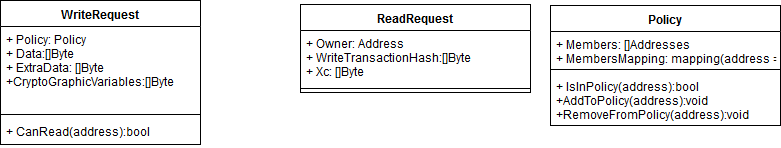
\includegraphics[width=1\textwidth]{UML.png}
    \caption{An UML description of the main contract types and their respective variables and methods}
    \label{fig:UML of contracts}
\end{figure}

\subsection{Adapting the Calypso contracts to Ethereum}

% isn't the ZKP on the write requests for ByzCoin? e.g., the write proves that he knows the secret
% why is it "cumbersome"? state the options (e.g., implement curve operations in solidity is an option, but takes long time and cost a lot of gas, or change the go implementation to use the ethereum curve but maybe there are no good libraries and it'll be difficult to compare two different implementations later when the curves are different)
% there is a paper that says it's not practical to implement your own curve operations in solidity because you hit the block gas limit, i can't remember what it is now but we can try to find it on monday
There are some important distinctions when trying to emulate how the process works on ByzCoin when working with Ethereum. The most obvious example would be the Zero-knowledge proofs(ZKP) that Byzcoin uses when trying to add a write transaction to a block. There are some methods of performing ZKP on Ethereum, most notably the Zk-Snarc\footnote{Here is an article by Vitalik Buterin on the subject https://medium.com/@VitalikButerin/zk-snarks-under-the-hood-b33151a013f6} approach, but most of these methods are defined over a different curve than the one Calypso and ByzCoin use and it proved too cumbersome to adjust these ZKP methods to the Ethereum implementation of Calypso.

Implementing Zero-Knowledge proofs on Ethereum proved cumbersome for a variety of reasons. The first one obviously has to do with it being implemented over a different curve than Calypso but there are also gas related problems. There are built in implementations of the curve Ethereum uses in go so it would have been possible to translate the ZKP variables but that proved extremely expensive in gas. As demonstrated by McCorry, Toreini and Mehrnezhad\cite{Toreini2016RemovingTT}, the gas cost of performing an ZKP on Ethereum can easily exceed the gas limit of of a block on the main net making it extremely costly to add a write request to Ethereum.

There are no restrictions on what kind of contracts can be deployed on an Ethereum network. By that restriction, or lack thereof, there is no way to validate a read request before deployment. If there is enough ether on the account to deploy a read request, then it will get added to a block. To validate both writes and read an encapsulating Calypso contract was created. The purpose of the Calypso contract is to validate both writes and reads such that if a read and write pair is present and both have been validated and added to a valid block. The read and write request are logged and verified using the corresponding addresses.

\begin{figure}[H]
    \centering
    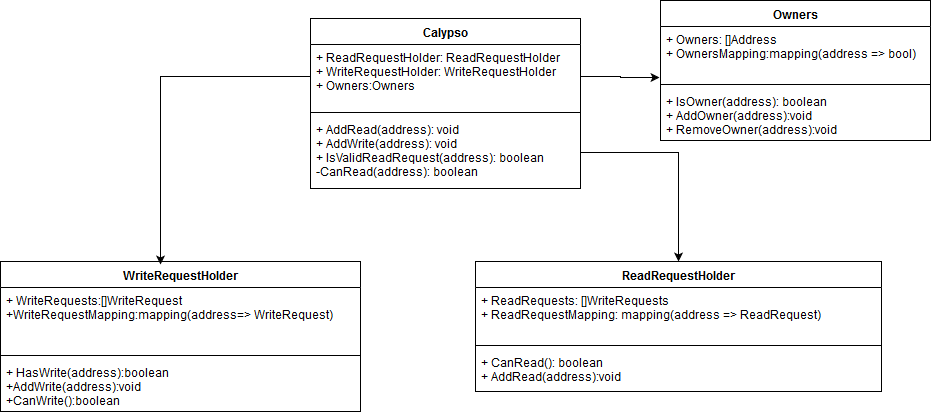
\includegraphics[width=1\textwidth]{UMLCalypso.png}
    \caption{Current Architecture of Calypso}
    \label{fig:calypsoStructure}
\end{figure}

\subsection{Working around the gas costs}

As stated before, a transaction in Ethereum is any form of action that changes the state of the blockchain. A state change can be transferring ether from one account to another, deploying a contract or changing the state of a contract, for example. Therefore, if someone wishes to change the state of the blockchain, they will have to be willing to pay a cost to the miners in the form of gas.

When developing the write and read request contracts, an important thing to keep in mind was to try and lower the gas cost as much as possible. There are multiple factors that affect the estimated gas cost of deploying a contract, such as the length of the contract, number of loops and how expensive some functions are like for example hash functions and signing functions. If a contract’s estimated gas cost is too much it can exceed the gas limit of a block or be extremely expensive to deploy.

% I feel this paragraph can be extended, it's an interesting problem and unique to this project. Can you give an example of the old contract and the new contract? maybe in pseudocode. then point out what exactly was changed
A problem that early implementations of the Calypso Ethereum platform faced is that the cost of deploying a contract exceeded the standard gas limit. The original implementation had little form of modularisation and used expensive methods to create unique identifiers such as the SHA256 hash function and nested data structures which is not  fully supported by Solidity except on the experimental release of the solidity compiler.  This approach was extremely problematic due to multiple reasons. One of those reasons being that the SHA256 hashing functions is a really expensive function to compute and it not only increased the cost of deploying the original Calypso contract but made indexing a write request very expensive as well. To solve this the Calypso contract had to be broken down into smaller components and a new way of indexing write and read requests had to be thought of.

\begin{figure}[H]
    \centering
    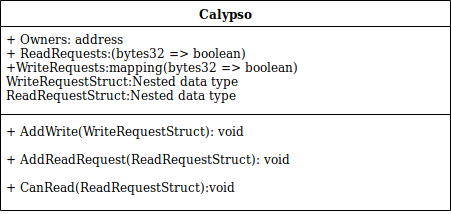
\includegraphics[width=1\textwidth]{OldCalypsoso.png}
    \caption{Old Architecture of Calypso}
    \label{fig:calypsoStructure}
\end{figure}

In this old contract, the add functions performed SHA256 hashing on the contents of the write and read requests and checked if they belonged in  a mapping. This was an expensive job to perform since it involved hashing on the  blockchain and the data of the requests had to be bundled together using the Ethereum ABI. Contrast this to the the new Calypso where the contract has been broken down  to contracts and sub-contracts and there is no longer any hashing of the data involved. This allowed to keep the amount of computations needed to deploy and add a request significantly. 


\subsection{Testing smart contracts}

% not sure whether I understood, so the web3 API is for unit tests, and the Truffle framework is more for integration testing, because it needs an Ethereum network. maybe clarify those points if that's true
After writing the write and read requests and constructing the Calypso contract, then the smart contracts had to be tested, both as units and integrated together. The web3 API provides a Javascript like console environment to both interact with and deploy smart contracts on an Ethereum network. It works great for when trying to debug a contract but that method can be rather cumbersome when trying to test functionality that requires multiple contracts and contract calls.

When testing the functionality of the contracts in isolation, being not as a part of an integrated system like Calypso, I used the Truffle node.js framework for testing the contract methods and making sure that everything was getting logged properly and the logic of the contracts was sound on the Ganache test network. When debugging a particular function that was behaving incorrectly or in a weird way I used the Web3 API to get a more hands on feeling on what was going wrong. 

To create an automatic test suite, I used the node.js Ethereum testing framework Truffle. Truffle allows for writing tests for Smart contracts in Solidity and javascript. Truffle allows for a lot of flexibility when it comes to testing. When testing the how contracts interact with each other it is possible to write tests in Solidity using truffle and when testing how contracts respond to user interaction. Truffle on its own is not sufficient for testing smart contracts. When configuring a testing suite using truffle, an Ethereum network must be provided for deploying smart contracts to. 

There are many open test nets available, such as the ropsten testnet, that allow for any account to have as much Ether as required and the ether has no real monetary value. This option is great for trying to determine if the smart contracts work as intended in a commercial environment, but it has a major drawback. When trying to deploy a smart contract to a non-local test net, the tests will have to wait for the transaction of the deployed contract has been added to a valid block. The time required to wait for a transaction to be added a block can vary greatly depending on the amount of traffic on the testnet and setting the block timer to a low value is not possible. Early on in the development stages, when there were a lot of changes between tests, and the changes were often rather significant, the open test nets were not a good option.

% what proved to be problematic?
%Explained later on.
The makers of the Truffle framework made the Ethereum client Ganache which allows for running a local Ethereum network. Ganache allows for a lot of tweaking of the setting of the network such as gas price, gas limit, block speed and the initial state of accounts on the network. This allowed for rapid development during the early stages of development, but did prove problematic once doing more sophisticated integration tests with the Calypso framework.

% the paragraphs above described all the options, can you write a paragraph for what you did for testing? 

\section{Integrating Calypso with Ethereum}
\subsection{Write requests}
% clarify that the CreateLTS stuff is only done once, both in the description and in the diagram. future write requests can re-use the old LTS ID.
Creating a write request in the Ethereum implementation is very similar to creating a write request in the original implementation of Calypso. Initially, the user will create a Long-term secret(LTS) and get the LTS reply. In addition to the usual variables stored by the secret-management cothority(SMC), the Ethereum implementation also stores the key-value pair of LTS ID as the key and an Ethereum address as the value. The Ethereum address corresponds to the Calypso contract where the Write request is indexed. After obtaining the LTS reply, the user can use the LTSID to make new write requests.When a new Write is issued using the data supplied to the client by the user, just like in the original Calypso, with an important distinction. Since there is no concept of a darc in Ethereum, creating a write request can’t be reliant on the same darc method as previously. Instead of a darc based ID, the write is made using the address of a policy contract and by marshalling the address to a slice of bytes and then added to the ZKP much in the same way as the darc ID. 

Having made a write request, the next step is to deploy a write request to Ethereum. Using the Calypso client, deploying a write request is a two-step process. First the client will deploy a write request to Ethereum and will be returned with a transaction and the address of the deployed write request. Then the client will log the newly deployed write request to the specified Calypso contract and wait for that transaction to be added to a valid block. The user will then be presented with the address of the write and the hash of the transaction of  the write request being logged to the Calypso contract.

% isn't the secret management cothority that does the LTS stuff? in the diagram it's "Access control cothority"
% what is IndexWrite?
\begin{figure}[H]
    \centering
    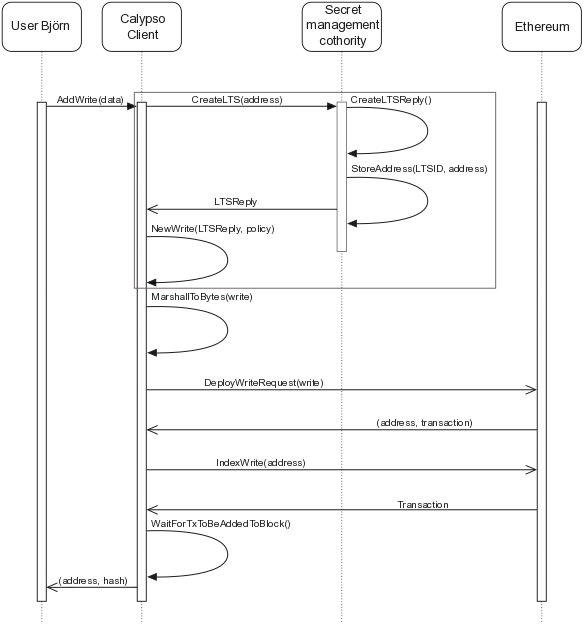
\includegraphics[width=1\textwidth]{NewWriteSequence.png}
    \caption{An UML describing the sequence of adding a write request}
    \label{fig:ReadRequestSequenceDiagram}
\end{figure}

\subsection{Read requests}
A Calypso Ethereum read request is essentially the same as a read request from the ByzCoin implementation with slight differences. The read request has the address of the corresponding write request it is requesting to read, the address of the account that issued the read request, public key of the reader and the hash of the transaction of the write request being added to Calypso.

Adding a read request to an Ethereum blockchain has a different process than adding a read request to ByzCoin. In ByzCoin, the read request will be validated against the policy of the Write request as part of the validation process. Since read requests can’t be validated against the policy on Ethereum before being deployed. Therefore, the client goes through the same two step process as with a write request.

% give references to the paper
Another important distinction between how read request are deployed is the aforementioned lack of ZKP on Ethereum. Since Ethereum does not have a working implementation of elliptic curve ed25519, implementing a Zero-Knowledge proof would be extremely difficult. A proof of concept that writing a ZKP on ethereum in raw Solidity code is possible is the work done by McCorry, Toreini and Mehrnezhad\cite{Toreini2016RemovingTT}. This approach has a few drawbacks which made it not a good option for the Calypso Ethereum implementation. The most significant drawback being that it is implemented over a different elliptic curve than the Calypso framework. Making it a necessary requirement to refactor the existing cryptographic codebase to work with another elliptic curve. Another significant drawback is the gas cost of an ZKP. The gas cost of running cryptographic functions on an  Ethereum network are really high, as illustrated by McCorry, Toreini and Mehrnezhad\cite{Toreini2016RemovingTT}. This is a major drawback since it would increase the monetary cost significantly of adding a write request.  With these drawbacks in mind an alternative solution had to be thought of.

When issuing a read request using the Calypso Ethereum client, the user must provide the address of a write request, the transaction hash of the Write request being indexed. The client will then validate that the write request has been indexed and that the transaction has been mined and added to a valid block. If the transaction was valid then it will make a call to the Ethereum network to retrieve a copy of the write request. Then it will verify the ZKP proof locally and if the ZKP passes then it will proceed to add the read request to Ethereum as mentioned previously.

% what is IndexRead?
\begin{figure}[H]
    \centering
    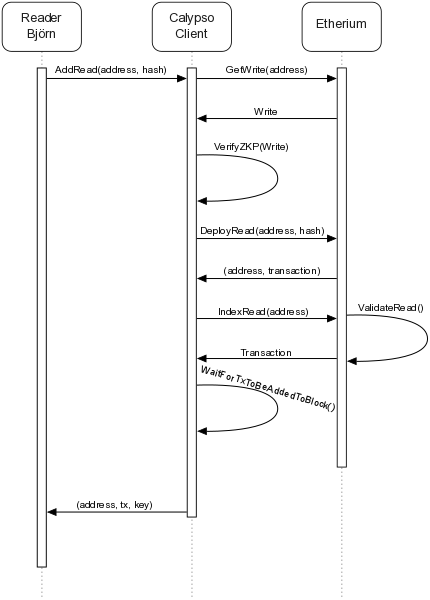
\includegraphics[width=1\textwidth]{NewReadSequence.png}
    \caption{An UML describing the sequence of adding a read request}
    \label{fig:ReadRequestSequenceDiagram}
\end{figure}

\subsection{Decrypt key process}
The decrypt key process is both similar and different from the original implementation. The off-chain parts of Calypso were for the most part the same except that the Calypso address where the write and read are logged is stored using the LTSID of the write request. When passing the decrypt key parameters to the decrypt key service function, the difference in what is passed is that in the original implementation of Calypso the decryptkey struct has the byzcoin write and read ID while in the Ethereum implementation of Calypso the corresponding addresses of the write and read contracts along with the hash of the transaction of the read being logged on Calypso.

First the process will fetch a copy of the write and read contracts from an Ethereum network. It will compare that the address stored in the read request is the same address as the write address presented to the decrypt key function. It will then get the hash of the write request from the read request and check that both the read and the write have been validated and added to a valid block on the Ethereum network. After validating that these addresses are valid and logged, the decryption moves as intended and the only alteration would be that in the verify re-encryption parts of the decryption process 

\section{Performance}
When assessing the performance of Calypso, there are a few metrics that can be examined. Metrics such as latency, gas cost, number of transactions in a block and data retrieval are all metrics that are important to examine, but can have greatly varying results depending on what kind of Ethereum network they are being tested on. 

\subsection{Choosing the performance testing network}
% it's not that ByzCoin has no users, but the current implementation is a permissioned blockchain.
% maybe change the title to "Choosing the performance testing network" because, ideally, we'd like to compare ByzCoin with a permissioned ethereum network for it to be fair, but due to the problems that you mentioned below, it was decided to do it on Ropsten testnet
During the performance evaluation phase of implementing Ethereum Calypso, there were a few difficulties that arose when trying to compare the new implementation to the previous one. It would be ideal to test the system on a commercial network of both ByzCoin and Calypso but that presents a big problem. Currently, the networks that are running ByzCoin are permissioned and can't be easily compared to the current Ethereum networks available that are not permissioned.

The first problem that arose was when trying to use the Ganache local Ethereum network with a custom block timer. The Ganache client worked when using it with a block timer of zero seconds but if the block timer became non zero or if a hash of a transaction had to be validated, it stopped working. Since the Ganache block mining algorithm was non-probabilistic and does not follow the conventional blockchain proof-of-work scheme, trying to validate a hash of a transaction on Ganache just returns an error. These are well documented flaws with Ganache which made it a non suitable platform for when the Ethereum implementation of Calypso became more complex.

All of the official Ethereum clients, fx eth, geth, parity, offer to be able to set up a local private network. This seemed to be the ideal solution since it would be using the most popular client for running Ethereum on a node and should have given accurate results. Setting up the network took a bit of time and there were some difficulties with the computers that the project being developed on not being good enough to mine if the difficulty was too hard. When the setup was done and the mining node process had been configured such that it was possible to send transactions to that node to be mined and the accounts to be tested with had been funded another problem arose. All transactions that were made not by the mining node were stuck in a pending state and were never added to a valid block. This turned out to be a problem with the eth clients when running on a private network. This would not have been a problem if the tests had only involved measuring metrics such as latency and gas cost but if the measurements required having to wait for a block to be mined or required multiple consequent transactions from the same account.

Due to these limitations, when trying to get a fair comparison proved to be almost impossible. Therefore, all of the measurements mentioned here on forward were performed on the Ropsten test net since it proved to be the most reliable.

\subsection{Gas performance}
Gas is the most independent from what kind of network is being of all the metrics. For Calypso, this concerns primarily the cost of deploying a write or a read request and indexing them in the Calypso contract and deploying a policy and updating it. The cost of deploying the Calypso contract and its helper contracts should be considered a one-time cost since it is mainly there for setup. 

The size of a read request is always the same and consequently the gas cost of adding a read request has a very low variance.

% can you put the gas prices in some context? like how much ether and how much USD/EUR/CHF are these gas prices?
% what does the Y axis say?
% usually i use .svg or .pdf files for graphs in latex so the quality stays high if latex decides to stretch the graph
\begin{figure}[H]
    \centering
    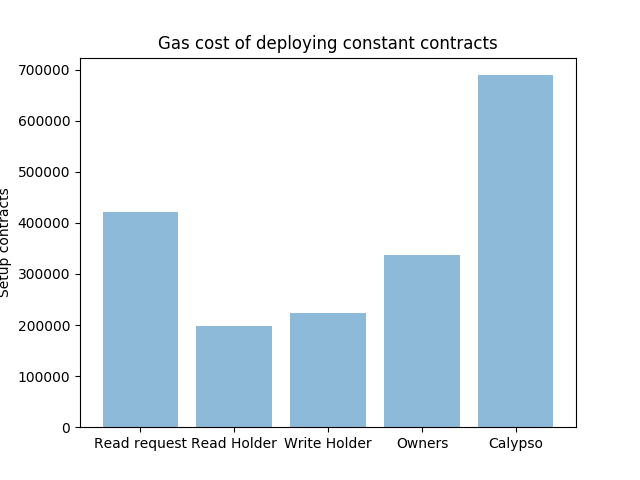
\includegraphics[width=1\textwidth]{ConstantGasCost.png}
    \caption{Different gas prices}
    \label{fig:contractsGasprices}
\end{figure}

As the size of the data that is to be stored in a write request increases, the gas cost increases. The gas cost increases approximately linearly as the size of the data increases. The figure below illustrates how the gas cost increases as the data size increases. 

% how many measurements did you do? it'd be nice to see some dots or crosses on the line
\begin{figure}[H]
    \centering
    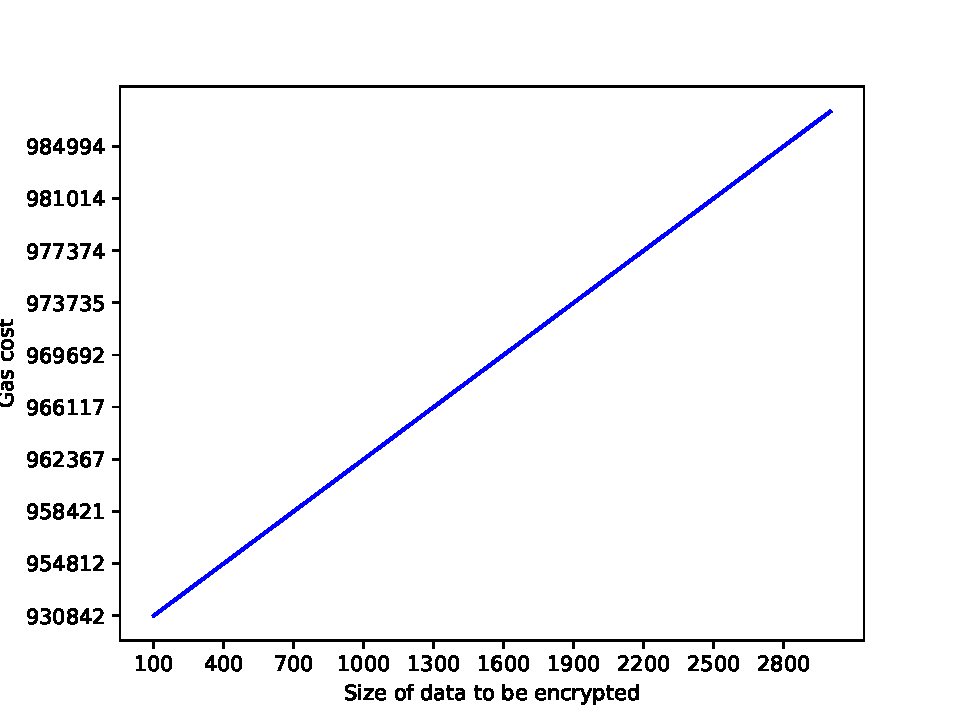
\includegraphics[width=1\textwidth]{WriteGasData.pdf}
    \caption{Gas cost as data size increases}
    \label{fig:contractsGasprices}
\end{figure}

A requirement for the policy is to both be of dynamic size and to be able to be updated on the fly. Adding to the policy and increasing the initial state of the policy grow in gas cost in a very similar way since in both cases, addresses are being indexed in a mapping. The figure below illustrates how the gas cost of the policy increases as the number of addresses to be indexed increases.

% how many measurements did you do? it'd be nice to see some dots or crosses on the line
\begin{figure}[H]
    \centering
    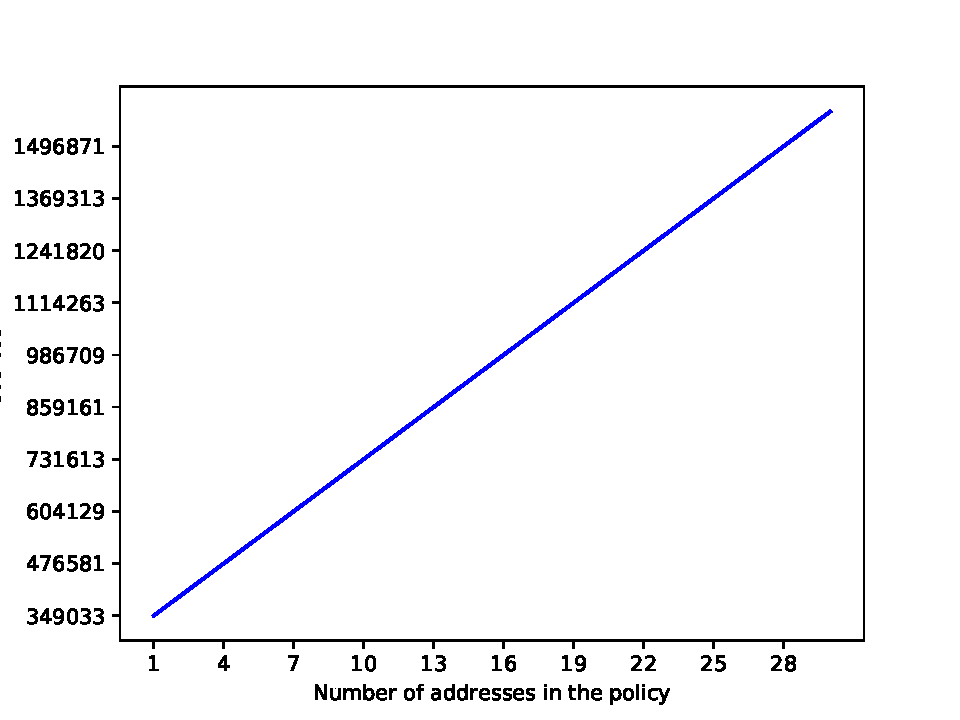
\includegraphics[width=0.8\textwidth]{PolicyGasData.pdf}
    \caption{Gas cost as number of addresses increases in the policy}
    \label{fig:contractsGasprices}
\end{figure}

\subsection{Timing performance}\
When assessing the timing performance of the system the factors taken into account were, how long does it take for a transaction to be added to a block, and how much time has to pass before it is possible to access the data in a write or read request.

% doesn't the difficulty change over time too? like if there are more miners then the difficulty increases
The time it takes for a transaction is heavily dependent on the difficulty of the network. The difficulty is usually set in the genesis json file of the genesis block of a blockchain and can vary greatly between different networks. Therefore, there were not any measurements made on this. 

% what do you mean by commercial network?
When measuring how long it takes to deploy a smart contract and how long it takes to retrieve the data, an observation was made that as long as you have the address of the contract it is possible to retrieve the data. Therefore when measuring how long it takes to be able to retrieve data from a deployed contract, you just have to measure how long does it take to receive the address of a deployed contract. Important to note that these numbers are heavily influenced by latency. The figure below demonstrates how much variance on latency there is when using a commercial network\footnote{Commercial network in the sense that it is used by a large number of people concurrently independently of each other for commercial purposes in a distributed network.}.

% can you explain a bit why the results look like this? it seems mostly are between 0 and 4 seconds which don't depend on the data size, but there are some outliers. and the outliers depend on the data size. perhaps these outliers are pushed to later blocks because they're too big?
\begin{figure}[H]
    \centering
    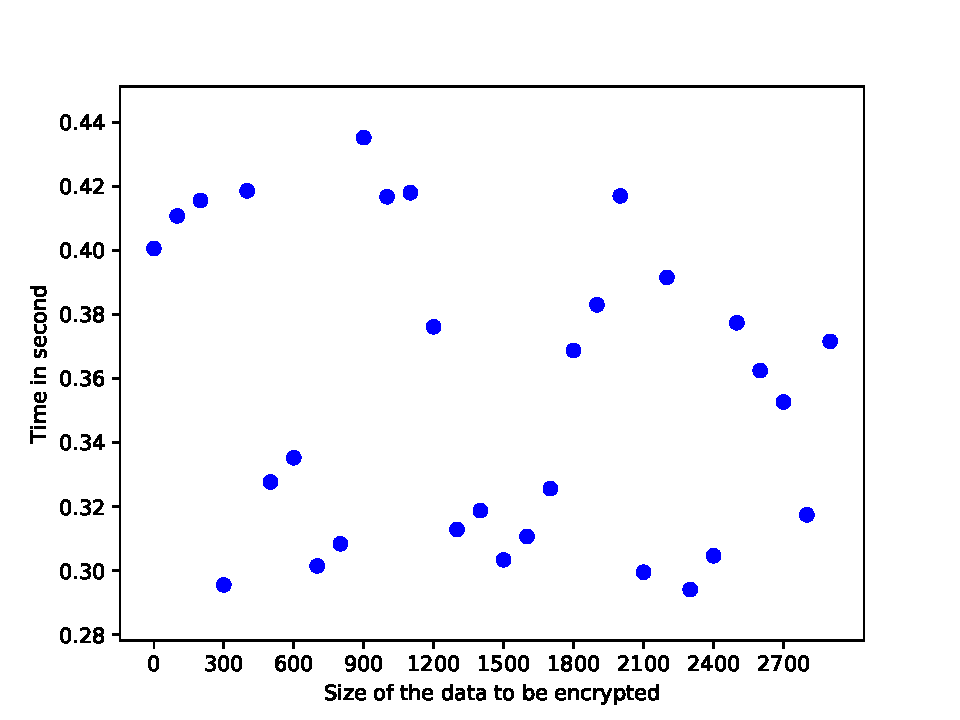
\includegraphics[width=1\textwidth]{WriteTimeData.pdf}
    \caption{Time until address is received}
    \label{fig:contractsGasprices}
\end{figure}

\subsection{Number of transactions in a block}

One of the methods that can give a good direct comparison between the ByzCoin and Ethereum is how many transaction can be added to a block. There are many factors that come into play, for example block difficulty. Like stated earlier, it was not possible, as of writing this, to get a fair comparison between the two implementation in these matters. There are methods that should give a pretty good estimate of how many blocks can be added to a block on a network. The gas limit of an Ethereum network serves as a metric of how many transactions can be added to a block.

Gas limit is a metric that indicates the maximum amount of transactions that can be added to a block. Transactions can have great variance in how much their gas cost is and when testing on a test net, the amount of transactions added, be it either deploying a write or a read request, can have insane variance due to competition from other participants in the network trying to get their transactions added. Since the amount of how many transactions is heavily influenced by both the gas limit and by making the assumption that the block difficulty is sufficiently difficult such that it should be possible to perform enough transactions before a block is found, the total amount of writes that can fit in a block should scale linearly for a constant data size while the amount of read request that fit in a block should scale linearly with the gas limit.
\begin{equation}
    TxCount = \floor*{\frac{gaslimit}{gascostoftransaction}}
    \label{eq:Equation for gas cost}
\end{equation}

% can you give an example of how many read/write requests that this tranlates to? e.g., if it's 50/50 read and write, how many tx can we do? if it's 90% read 10% write, how many tx can we do? (these percentages are from some kind of standard benchmark, i can find it id you'd like)
% also, if you have TxCount, you can also compute the transaction rate, and compare it to ByzCoin

\section{Future work}

% there is like an enterprise version of ethereum, I've only heard of the name, not sure whether it has any differences, but I imagine it is designed for permissioned environments. if that's the case, another direction for future work would be to use that. 

For anyone continuing work on this project my suggestion would be to implement a way to perform ZKP on Ethereum that is possible to implement on Ethereum and integrate with Calypso. The ZKP is a fundamental aspect of Calypso and it would help mitigate the amount of spam on the Ethereum network. There are already known examples of ZKP on Ethereum but those solutions either require re-structuring the threshold cryptographic system of Calypso to be defined on another elliptic curve or to implement a ZKP in Solidity over elliptic curve ed25519,

Another improvement would be to set up an automatic test suite on Ethereum. As mentioned previously, the options for testing on a local controlled Ethereum network were very limited and had known problems. Even if they had not had these problems, every time a configuration had to be changed a new blockchain had to be made manually and accounts prefunded before any transactions could be added. Therefore, I think an automatic test suite that can be easily configured on the fly is a great avenue for future improvement on this project.

A possible field of exploration could also be on the subject on enterprise Ethereum. Enterprise Ethereum is an organization comprised of many large corparations working together to create an Ethereum standard for corporations to use. An interesting use case could be to test if Calypso can be properly integrated with enterprise Ethereum and maybe get a more fair comparison between it and ByzCoin.

\section{Conclusion}

Ethereum shows a lot of promise. The Ethereum virtual machine has a lot of flexibility for writing smart contracts and interacting with an Ethereum network using Go is both well supported and easily accessible. With that being said, I still think the limitations of Ethereum currently make it not a suitable blockchain platform for Calypso as it stands. Both due to lack of support of the ZKP and the inability to get a good direct comparison between performances of the two implementations.


\newpage
\bibliographystyle{plain}
\bibliography{ref.bib}

\end{document}
